% Source: inputs/original_02.pdf p.6 (printed 5-38), question 25 solution figure.
% Three panels k=1,2,3: unit circle center (0,1), O=(0,0), Z0=(0,2), Z,Z' on circle.
\usetikzlibrary{arrows.meta,calc}
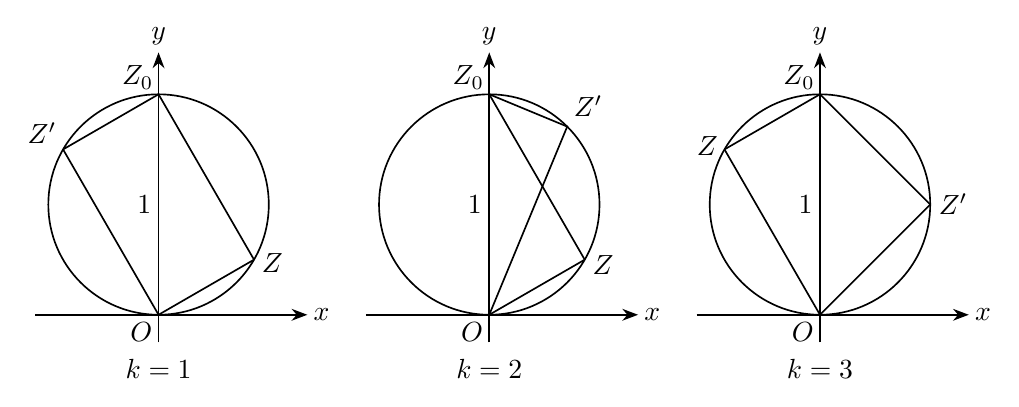
\begin{tikzpicture}[x=1.4cm,y=1.4cm,line width=.6pt,font=\normalsize,>=Stealth]
  \coordinate (O1) at (0,0);
  \coordinate (C1) at (0,1);
  \coordinate (Z0_1) at (0,2);
  \coordinate (Z1) at (0.866025,0.5);
  \coordinate (Zp1) at (-0.866025,1.5);

  \coordinate (O2) at (3,0);
  \coordinate (C2) at (3,1);
  \coordinate (Z0_2) at (3,2);
  \coordinate (Z2) at (3.866025,0.5);
  \coordinate (Zp2) at (3.707107,1.707107);

  \coordinate (O3) at (6,0);
  \coordinate (C3) at (6,1);
  \coordinate (Z0_3) at (6,2);
  \coordinate (Z3) at (5.133975,1.5);
  \coordinate (Zp3) at (7,1);

  \draw[->] (-1.12,0)--(1.35,0);
  \draw[->] (0,-0.25)--(0,2.38);
  \node[anchor=west,inner sep=0pt] at (1.40,0) {$x$};
  \node[anchor=south,inner sep=0pt] at (0,2.44) {$y$};
  \draw (C1) circle[radius=1];
  \draw (O1)--(Z1);
  \draw (O1)--(Zp1);
  \draw (Z0_1)--(Z1);
  \draw (Z0_1)--(Zp1);
  \node[anchor=south east,inner sep=0pt] at (-0.04,2.04) {$Z_0$};
  \node[anchor=west,inner sep=0pt] at (0.93,0.47) {$Z$};
  \node[anchor=south east,inner sep=0pt] at (-0.92,1.55) {$Z'$};
  \node[anchor=north east,inner sep=0pt] at (-0.05,-0.06) {$O$};
  \node[anchor=east,inner sep=0pt] at (-0.06,1) {$1$};
  \node[anchor=north,inner sep=0pt] at (0,-0.40) {$k=1$};

  \draw[->] (1.88,0)--(4.35,0);
  \draw[->] (3,-0.25)--(3,2.38);
  \node[anchor=west,inner sep=0pt] at (4.40,0) {$x$};
  \node[anchor=south,inner sep=0pt] at (3,2.44) {$y$};
  \draw (C2) circle[radius=1];
  \draw (O2)--(Z2);
  \draw (O2)--(Zp2);
  \draw (Z0_2)--(Z2);
  \draw (Z0_2)--(Zp2);
  \node[anchor=south east,inner sep=0pt] at (2.96,2.04) {$Z_0$};
  \node[anchor=west,inner sep=0pt] at (3.93,0.45) {$Z$};
  \node[anchor=south west,inner sep=0pt] at (3.76,1.79) {$Z'$};
  \node[anchor=north east,inner sep=0pt] at (2.95,-0.06) {$O$};
  \node[anchor=east,inner sep=0pt] at (2.94,1) {$1$};
  \node[anchor=north,inner sep=0pt] at (3,-0.40) {$k=2$};

  \draw[->] (4.88,0)--(7.35,0);
  \draw[->] (6,-0.25)--(6,2.38);
  \node[anchor=west,inner sep=0pt] at (7.40,0) {$x$};
  \node[anchor=south,inner sep=0pt] at (6,2.44) {$y$};
  \draw (C3) circle[radius=1];
  \draw (O3)--(Z3);
  \draw (O3)--(Zp3);
  \draw (Z0_3)--(Z3);
  \draw (Z0_3)--(Zp3);
  \node[anchor=south east,inner sep=0pt] at (5.96,2.04) {$Z_0$};
  \node[anchor=east,inner sep=0pt] at (5.08,1.53) {$Z$};
  \node[anchor=west,inner sep=0pt] at (7.07,1.0) {$Z'$};
  \node[anchor=north east,inner sep=0pt] at (5.95,-0.06) {$O$};
  \node[anchor=east,inner sep=0pt] at (5.94,1) {$1$};
  \node[anchor=north,inner sep=0pt] at (6,-0.40) {$k=3$};
\end{tikzpicture}
